\documentclass{beamer}

\usepackage{beamerthemesplit}
\usepackage{verbatim}
\usepackage[normalem]{ulem}

\usepackage{xcolor}

\usepackage{hyperref}

\definecolor{gold}{rgb}{1.,0.84,0.}
\definecolor{brightred}{rgb}{1.,0.4,0.4}
\definecolor{mygray}{RGB}{200,200,200}
\definecolor{lightsteelblue}{RGB}{176,196,222}
\definecolor{lightskyblue}{RGB}{135,206,250}
\definecolor{cadetblue}{RGB}{95,158,160}

\usetheme{default}
\usecolortheme{mule}

\usefonttheme{serif}

%\DeclareGraphicsExtensions{.pdf,.png,.jpg}

\newcommand{\mcal}{\textsc{metacalibration}}
\newcommand{\Mcal}{\textsc{Metacalibration}}

\newcommand{\mcalR}{\mbox{\boldmath $R$}}
\newcommand{\mcalRscalar}{\mbox{$R$}}

\newcommand{\mcalRmean}{\mbox{\boldmath $\langle R \rangle$}}
\newcommand{\mcalRscalarmean}{\mbox{$\langle R \rangle$}}

\newcommand{\mcalRpsf}{$R^{p}$}
\newcommand{\mcalRpsfnoise}{$R^{p}_\eta$}
\newcommand{\mcalRo}{\mbox{\boldmath $R_o$}}
\newcommand{\mcalRnoise}{\mbox{\boldmath $R_\eta$}}

\newcommand{\mcalRmeanalpha}{\mbox{\boldmath $\langle R_\alpha \rangle$}}
\newcommand{\mcalRmeanbeta}{\mbox{\boldmath $\langle R_\beta \rangle$}}

\newcommand{\mcalRg}{\mbox{\boldmath $R_\gamma$}}
\newcommand{\mcalRS}{\mbox{\boldmath $R_S$}}
\newcommand{\mcalRgmean}{\mbox{\boldmath $\langle R_\gamma \rangle$}}
\newcommand{\mcalRSmean}{\mbox{\boldmath $\langle R_S \rangle$}}

\newcommand{\mcalRtwopt}{\mbox{\boldmath $R^{2pt}$}}
\newcommand{\mcalRtwoptmean}{\mbox{\boldmath $\langle R^{2pt} \rangle$}}


\newcommand{\mcalRmodel}{\mbox{\boldmath $R^{model}$}}
\newcommand{\mcalRnoisemodel}{\mbox{\boldmath $R^{model}_\eta$}}


\newcommand{\vecg}{\mbox{\boldmath $\gamma$}}
\newcommand{\vest}{\mbox{\boldmath $e$}}

\newcommand{\snr}{$S/N$}
\newcommand{\snT}{$(S/N)_{\textrm{size}}$}
%\newcommand{\snT}{$\left( \frac{S}{N}\right)_{\textrm{size}}$}
\newcommand{\snflux}{$(S/N)_{\textrm{flux}}$}
%\newcommand{\snflux}{$\left( \frac{S}{N}\right)_{\textrm{flux}}$}

\newcommand{\lensfit}{\texttt{LENSFIT}}
\newcommand{\numba}{\texttt{Numba}}
\newcommand{\python}{\texttt{Python}}
\newcommand{\ngmix}{\texttt{ngmix}}
\newcommand{\ngmixer}{\texttt{ngmixer}}
\newcommand{\shear}{{\bf g}}
\newcommand{\redmapper}{redMaPPer}
\newcommand{\est}{$e$}


\newcommand{\prelim}{{\bf{\it Preliminary}}}

\newcommand{\uberseg}{{\color{lightsteelblue} {\"u}berseg}}
\newcommand{\MOF}{{\color{brightred}MOF}}


\title{Tests of the Scarlet and Multi-object Fitting Deblenders for
Weak Lensing Shear Recovery}
\author{Erin Sheldon and Lorena Mezini}
\institute{Brookhaven National Laboratory, Stony Brook University}

% http://texblog.net/latex-archive/plaintex/beamer-footline-frame-number/
% to add the page (frame ) number and not screw up the bottom line
% works for split themes?
\expandafter\def\expandafter\insertshorttitle\expandafter{%
      \insertshorttitle\hfill%
        \insertframenumber\,/\,\inserttotalframenumber}

% suppress navigation bar
\beamertemplatenavigationsymbolsempty
\setbeamertemplate{footline}{}

\begin{document}


\frame{\titlepage}

\frame
{
    \frametitle{Testing Scarlet for Shear Recovery}

    \begin{itemize}

        \item Motivation was to test Scarlet statistically for
            weak lensing shear recovery.
            
        \item Test in regime most interesting for weak lensing:  objects
            are small blobs after pixelization and smearing by the PSF.

        \item Use the Multi-Object Fitter (MOF) from Dark Energy Survey as a
            benchmark.  Needed a new implementation because original is not a
            library (Matt Becker using my ngmix package).

    \end{itemize}

}



\frame
{
    \frametitle{Scarlet Deblender Introduction}

    \begin{itemize}

        \item See Melchior et al. \url{https://arxiv.org/abs/1802.10157 }
            and talks yesterday.

        \item The number of objects, and nominal center for each object, are inputs.

        \item Every pixel is a parameter.


        \item Use constraints to reduce the dimensionality, e.g.
        \begin{itemize}
            \item Positivity (required)
            \item Monotonicity
            \item Symmetry
        \end{itemize}

    \end{itemize}

}

\frame
{

    \frametitle{Example Scarlet Deblend from HSC}

    %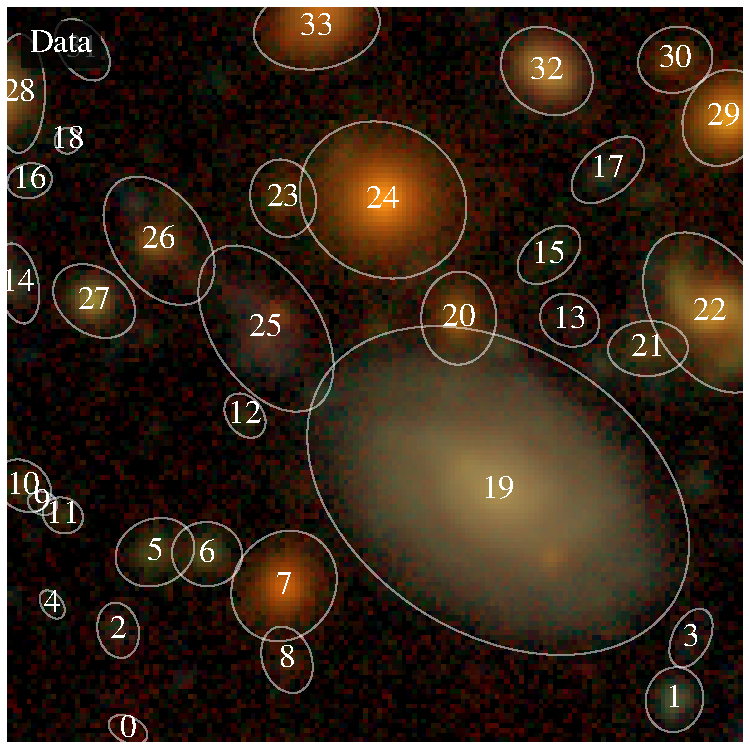
\includegraphics[width=.332\linewidth]{HSC_example_3_data}
    %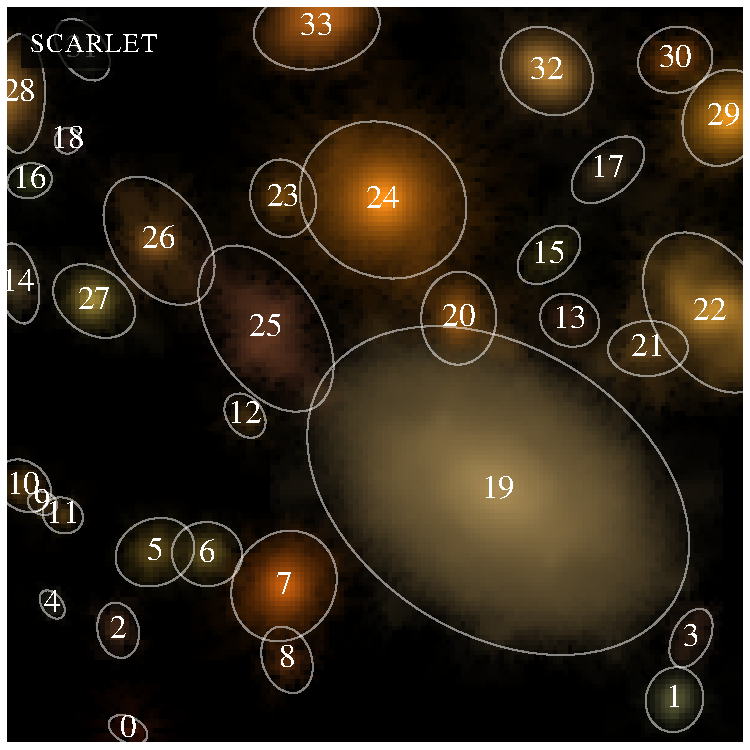
\includegraphics[width=.332\linewidth]{HSC_example_3_model}
    %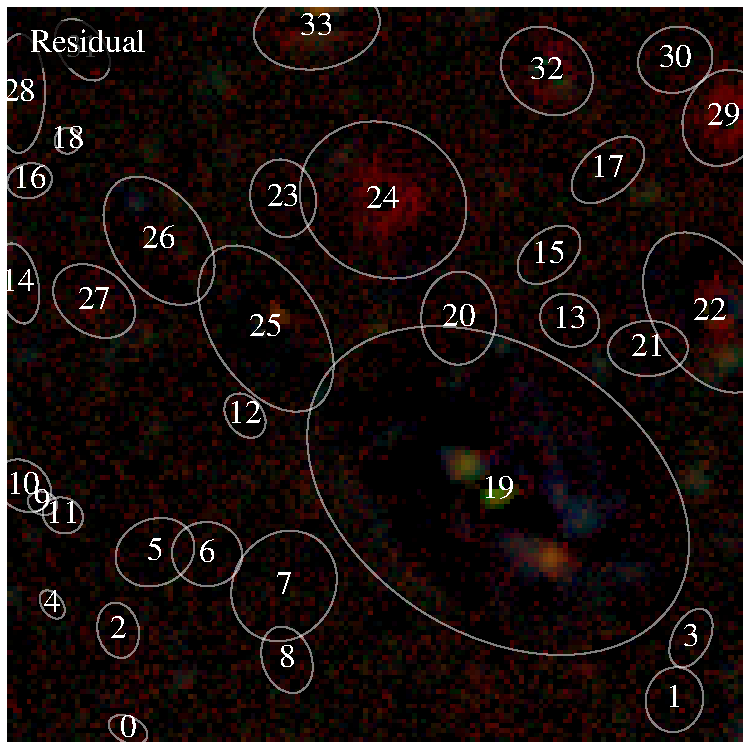
\includegraphics[width=.332\linewidth]{HSC_example_3_residual}

    \begin{center}
    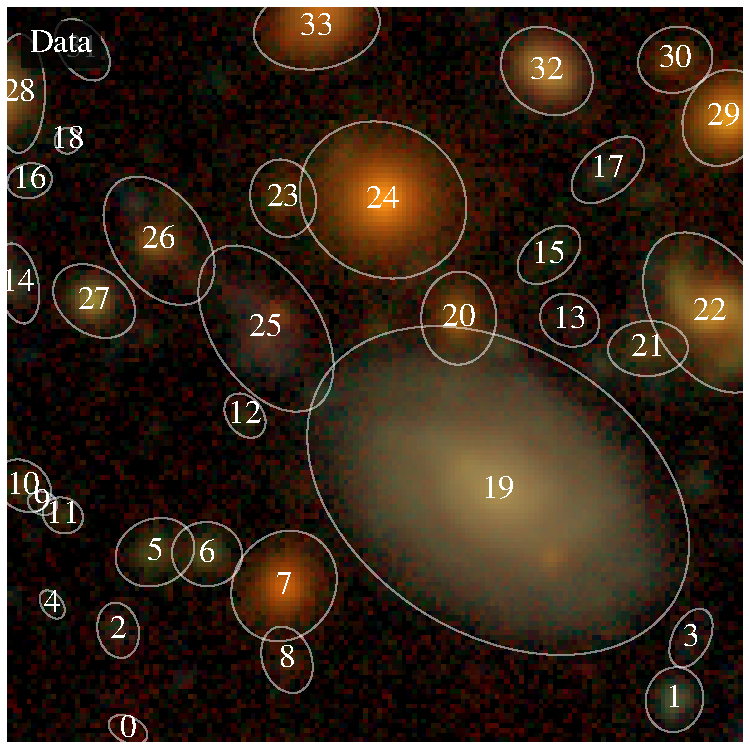
\includegraphics[width=.35\linewidth]{HSC_example_3_data}
    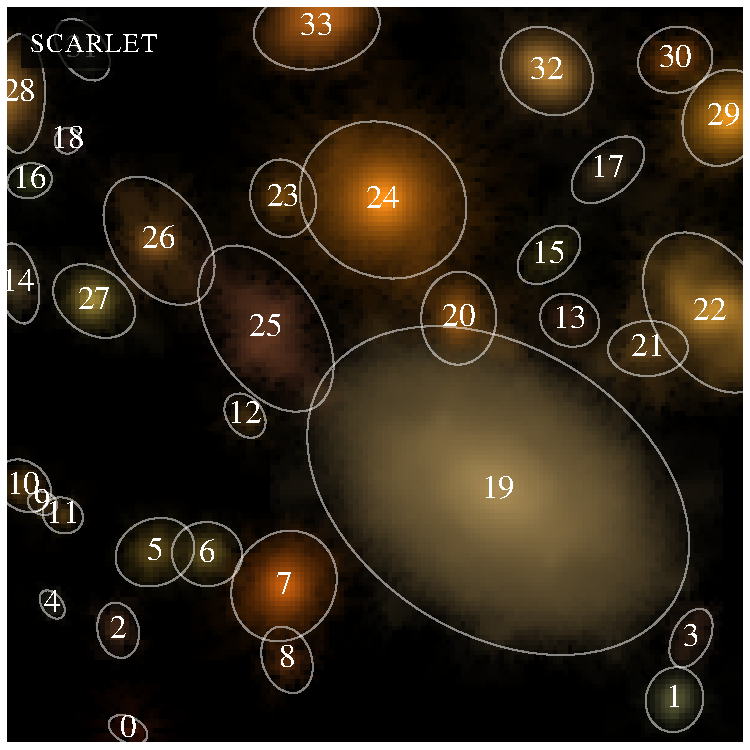
\includegraphics[width=.35\linewidth]{HSC_example_3_model}
    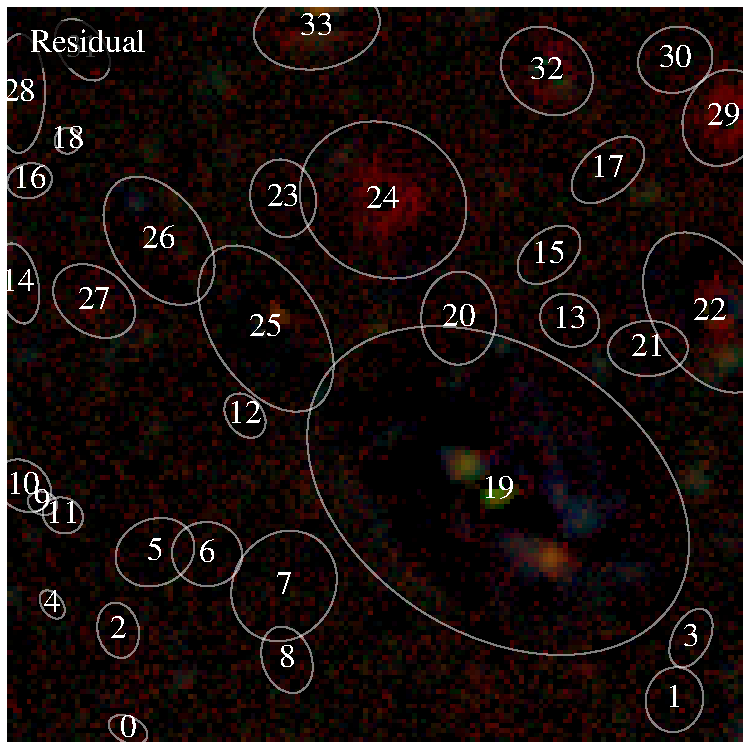
\includegraphics[width=.35\linewidth]{HSC_example_3_residual}
    \end{center}


}

\frame
{
    \frametitle{Multi-object Fitting Deblender (MOF)}

    \begin{itemize}

        \item New Implementation of the Dark Energy Survey MOF deblender
            (original Matt Becker using my \ngmix\ code base)

        \item Fit all objects in a blend simulateously
            with flexible models (original MOF was iterative)

        \item Model is bulge+disk, with both components
            the same size, ellipticity and center.

        \item Regularize some parameters to make the process stable.
            \begin{itemize}
                \item Shape
                \item Bulge fraction
                \item Center
                \item No regularization of size or fluxes needed.
            \end{itemize}

    \end{itemize}

}

\frame
{
    \frametitle{Multi-object Fitting}

    \begin{itemize}
            
        \item Can fit large groups simultaneously.

        \item In simulations, very stable, sub-percent failure rate even for
            large groups.

        \item I have fitted up to 225 objects. All of the 24 such groups I
            tried converged

    \end{itemize}

}


\frame
{
    \frametitle{Controlled Deblend Simulations for Shear Recovery}

    \begin{itemize}

        \item Simulate pairs of galaxies at various separations

        \item For what I will show, there is a ``central'' used
            to measure the shear.

        \item There is a ``neighbor'' which is twice as big and 33\% brighter.

        \item We have tried many models for these objects.  Shown here are
            examples for
            \begin{itemize}
                \item bulge+disk
                \item bulge has a different sizes, ellipticity, and
                    is offset from the disk center.
                \item Disk is scattered with knots of star formation.
                    
                \item These are not a good fit for the MOF model generally.

            \end{itemize}

    \end{itemize}

}

\frame
{
    \frametitle{Example Simulated Galaxies (Large)}

    \centering
    \includegraphics[width=0.7\linewidth]{{example-gals-007.pdf}}
}


\frame
{
    \frametitle{Example MOF de-blended pair. Low Noise.}

    \begin{center}
    \includegraphics[width=0.9\linewidth]{{bdk-N0.1-r07-example}.png}
    \end{center}

    Left is original, right is MOF deblended.
    \newline
    Can see residuals from ``knots'' of star formation.
}

\frame
{
    \frametitle{Example MOF de-blended pair. Medium Noise (S/N$\sim 50$.)}

    \begin{center}
    \includegraphics[width=0.9\linewidth]{{bdk-N10-r07-example}.png}
    \end{center}

    Left is original, right is MOF deblended.

}

\frame
{
    \frametitle{Multiplicative bias $m$ as a function of separation}

    \begin{center}
    \includegraphics[width=0.8\linewidth]{{bias_v_rad_mof_scar_bdk}.png}
    \end{center}


}

\frame
{
    \frametitle{Multiplicative bias $m$ (zoomed in)}

    \begin{center}
    \includegraphics[width=0.8\linewidth]{{bias_v_rad_mof_scar_bdk_zoom}.png}
    \end{center}


}

\frame
{
    \frametitle{Main Shear Test Results}

    \begin{itemize}

        \item MOF has expected behavior
            \begin{itemize}
                \item No bias for high S/N objects
                \item No bias at large separations
                \item Small bias for close separations and moderate S/N.
            \end{itemize}

        \item Scarlet shows surprising behavior
            \begin{itemize}
                \item Large bias at high S/N
                \item Unpredictable bias as a function of separation
                    at low S/N
            \end{itemize}

        \item We have been working closely with Peter and Fred to
            figure this out.

    \end{itemize}

}

\frame
{

    \frametitle{A Clue: Recovered Position Offsets, Relative to Truth}

    \begin{columns}
        \begin{column}{0.5\textwidth}
            \centering
            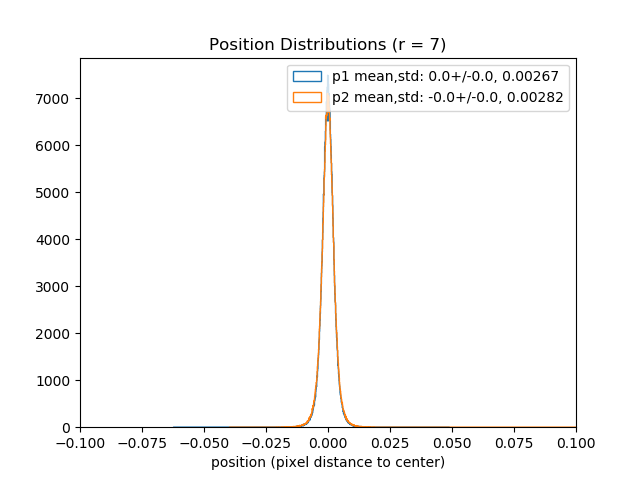
\includegraphics[width=\textwidth]{mof-posit-r7-lownoise.png}
            \newline
            MOF
        \end{column}
        \begin{column}{0.5\textwidth}
            \centering
            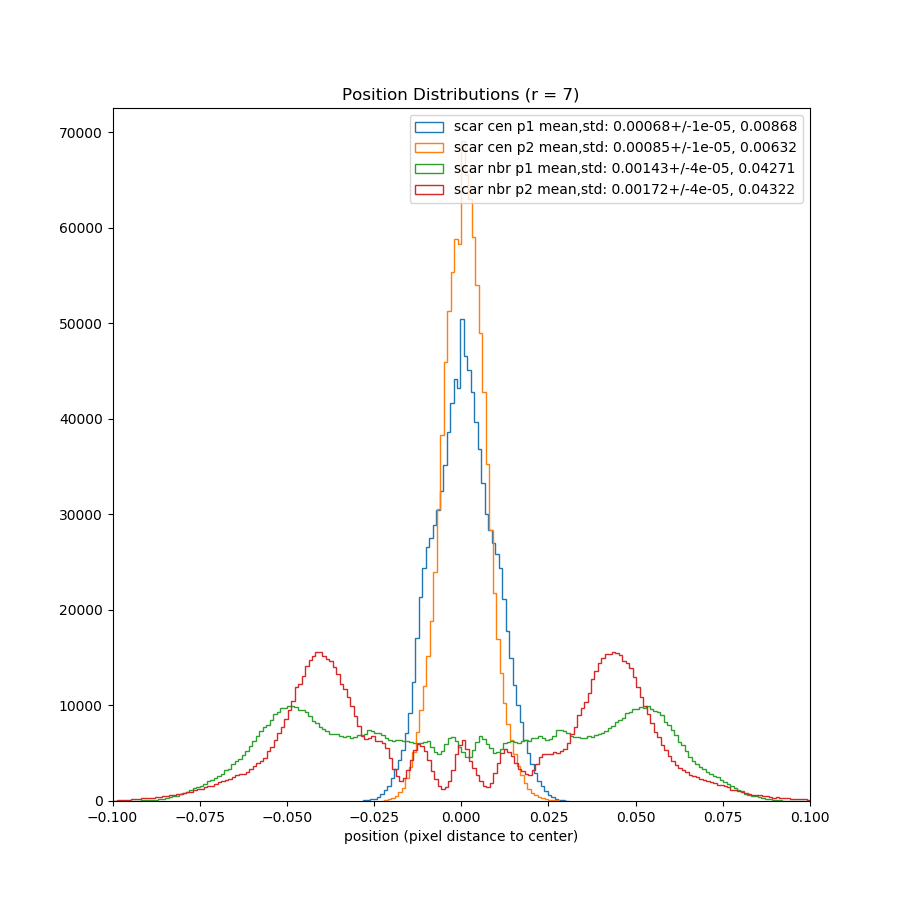
\includegraphics[width=\textwidth]{scar-posit-r7-lownoise.png}
            \newline
            Scarlet
        \end{column}
    \end{columns}

}

\frame
{
    \frametitle{Centering issues}

    \begin{itemize}

        \item The MOF behavior is as expected: the best-fit positions are
            centered on the truth with some Gaussian scatter.

        \item Scarlet positions look erratic.

        \item Not shown: sometimes the center can jump far outside the image,
            like $10^{10}$ pixels away.

        \item Fred and Peter think they understand this behavior and are
            working on a fix.

    \end{itemize}

}


\frame
{
    \frametitle{Summary}

    \begin{itemize}

        \item Scarlet is currently showing some surprising behavior
            for shear recovery.

        \item We are working with Fred and Peter to fix it.

        \item Lessons learned
            \begin{itemize}

                \item For weak lensing, simpler may be better.  Should we
                    adopt different constraints for Scarlet when
                    using it for weak lensing?

                \item Scarlet is very promising but if you want it to work for
                    your science case, then you need to test it!

                \item The scarlet developers are very responsive and
                    helpful.

            \end{itemize}

    \end{itemize}

}

\frame
{
    \frametitle{Extra Slides}

}

\frame
{
    \frametitle{Detection vs Deblending}

    \begin{itemize}

        \item For faint blobs detection is more of an issue
            than deblending.

        \item If you know the positioins of the objects in the
            field, MOF will produce a model with small residuals

        \item If the detection is imperfect, there will be
            large residuals, independent of the deblender or model
            that is fit.

    \end{itemize}

}

\frame
{
    \frametitle{Example Deblend}

        256 objects, 220 found by SExtractor
    \begin{center}
        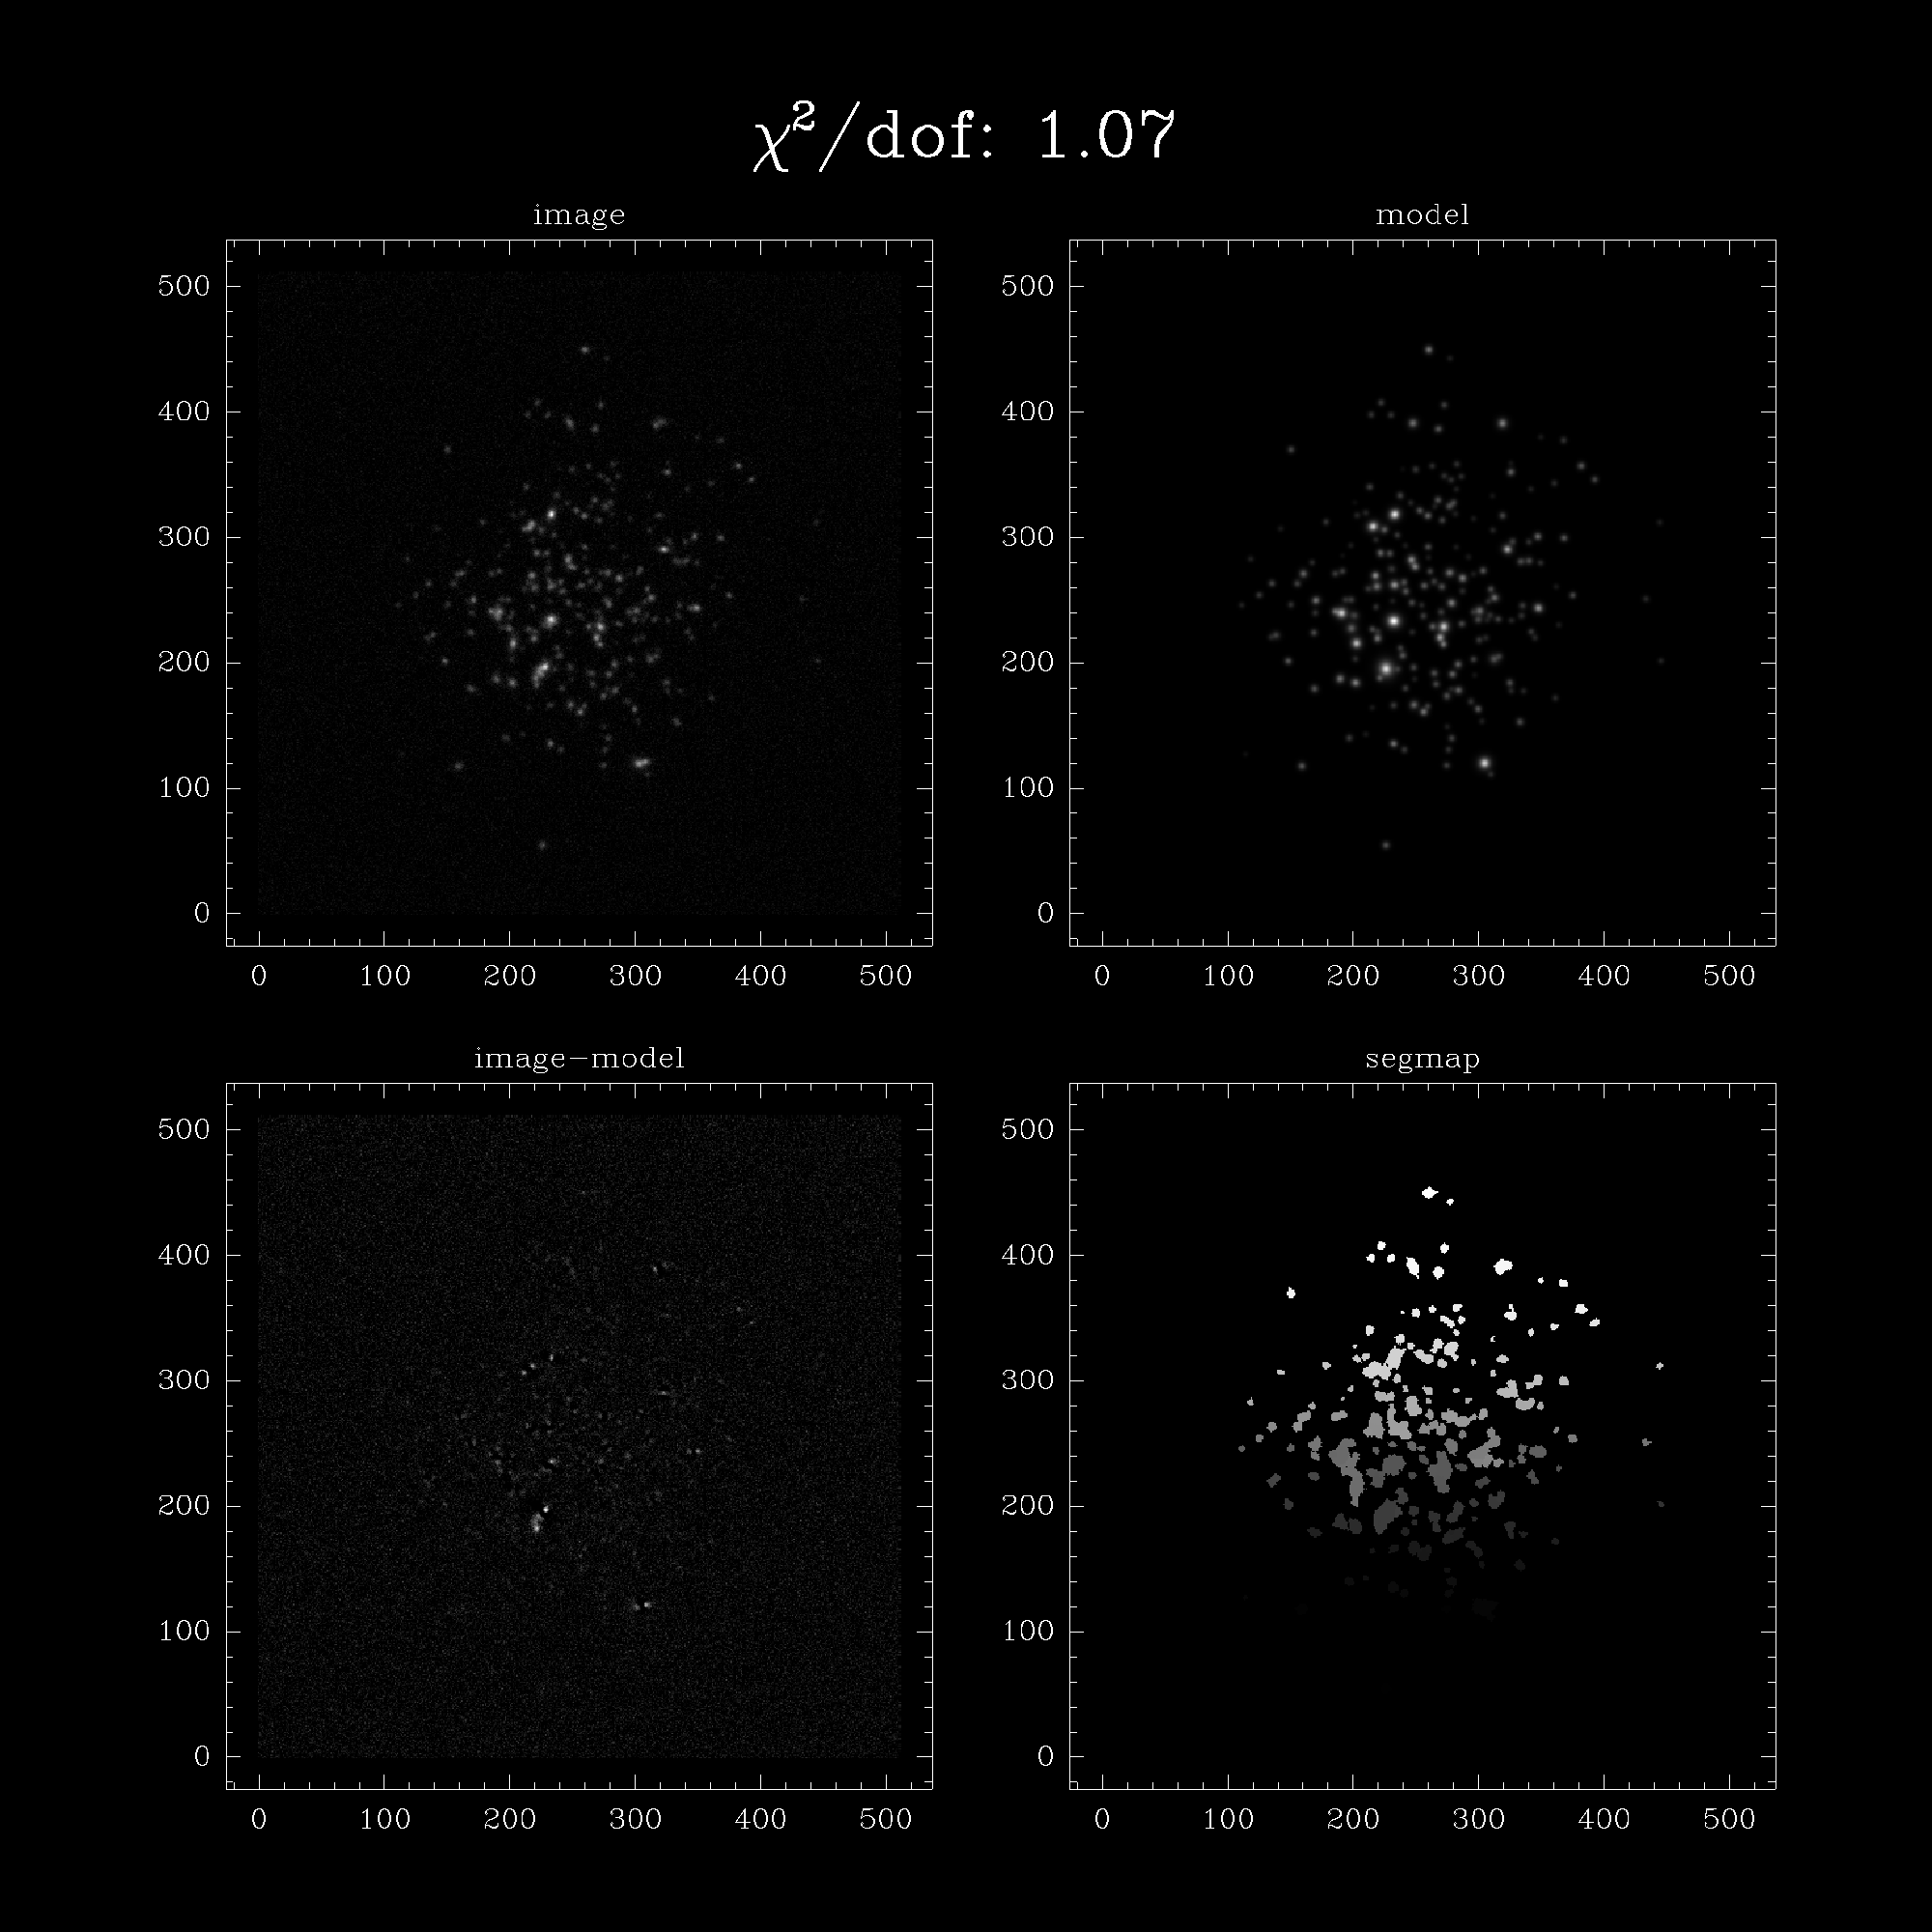
\includegraphics[trim={5cm 33cm 5cm 7cm},clip,width=\columnwidth]{diff-20855-000000.png}
    \end{center}
}

\frame
{
    \frametitle{Example Deblend}

        256 objects, 220 found by SExtractor
    \begin{center}
        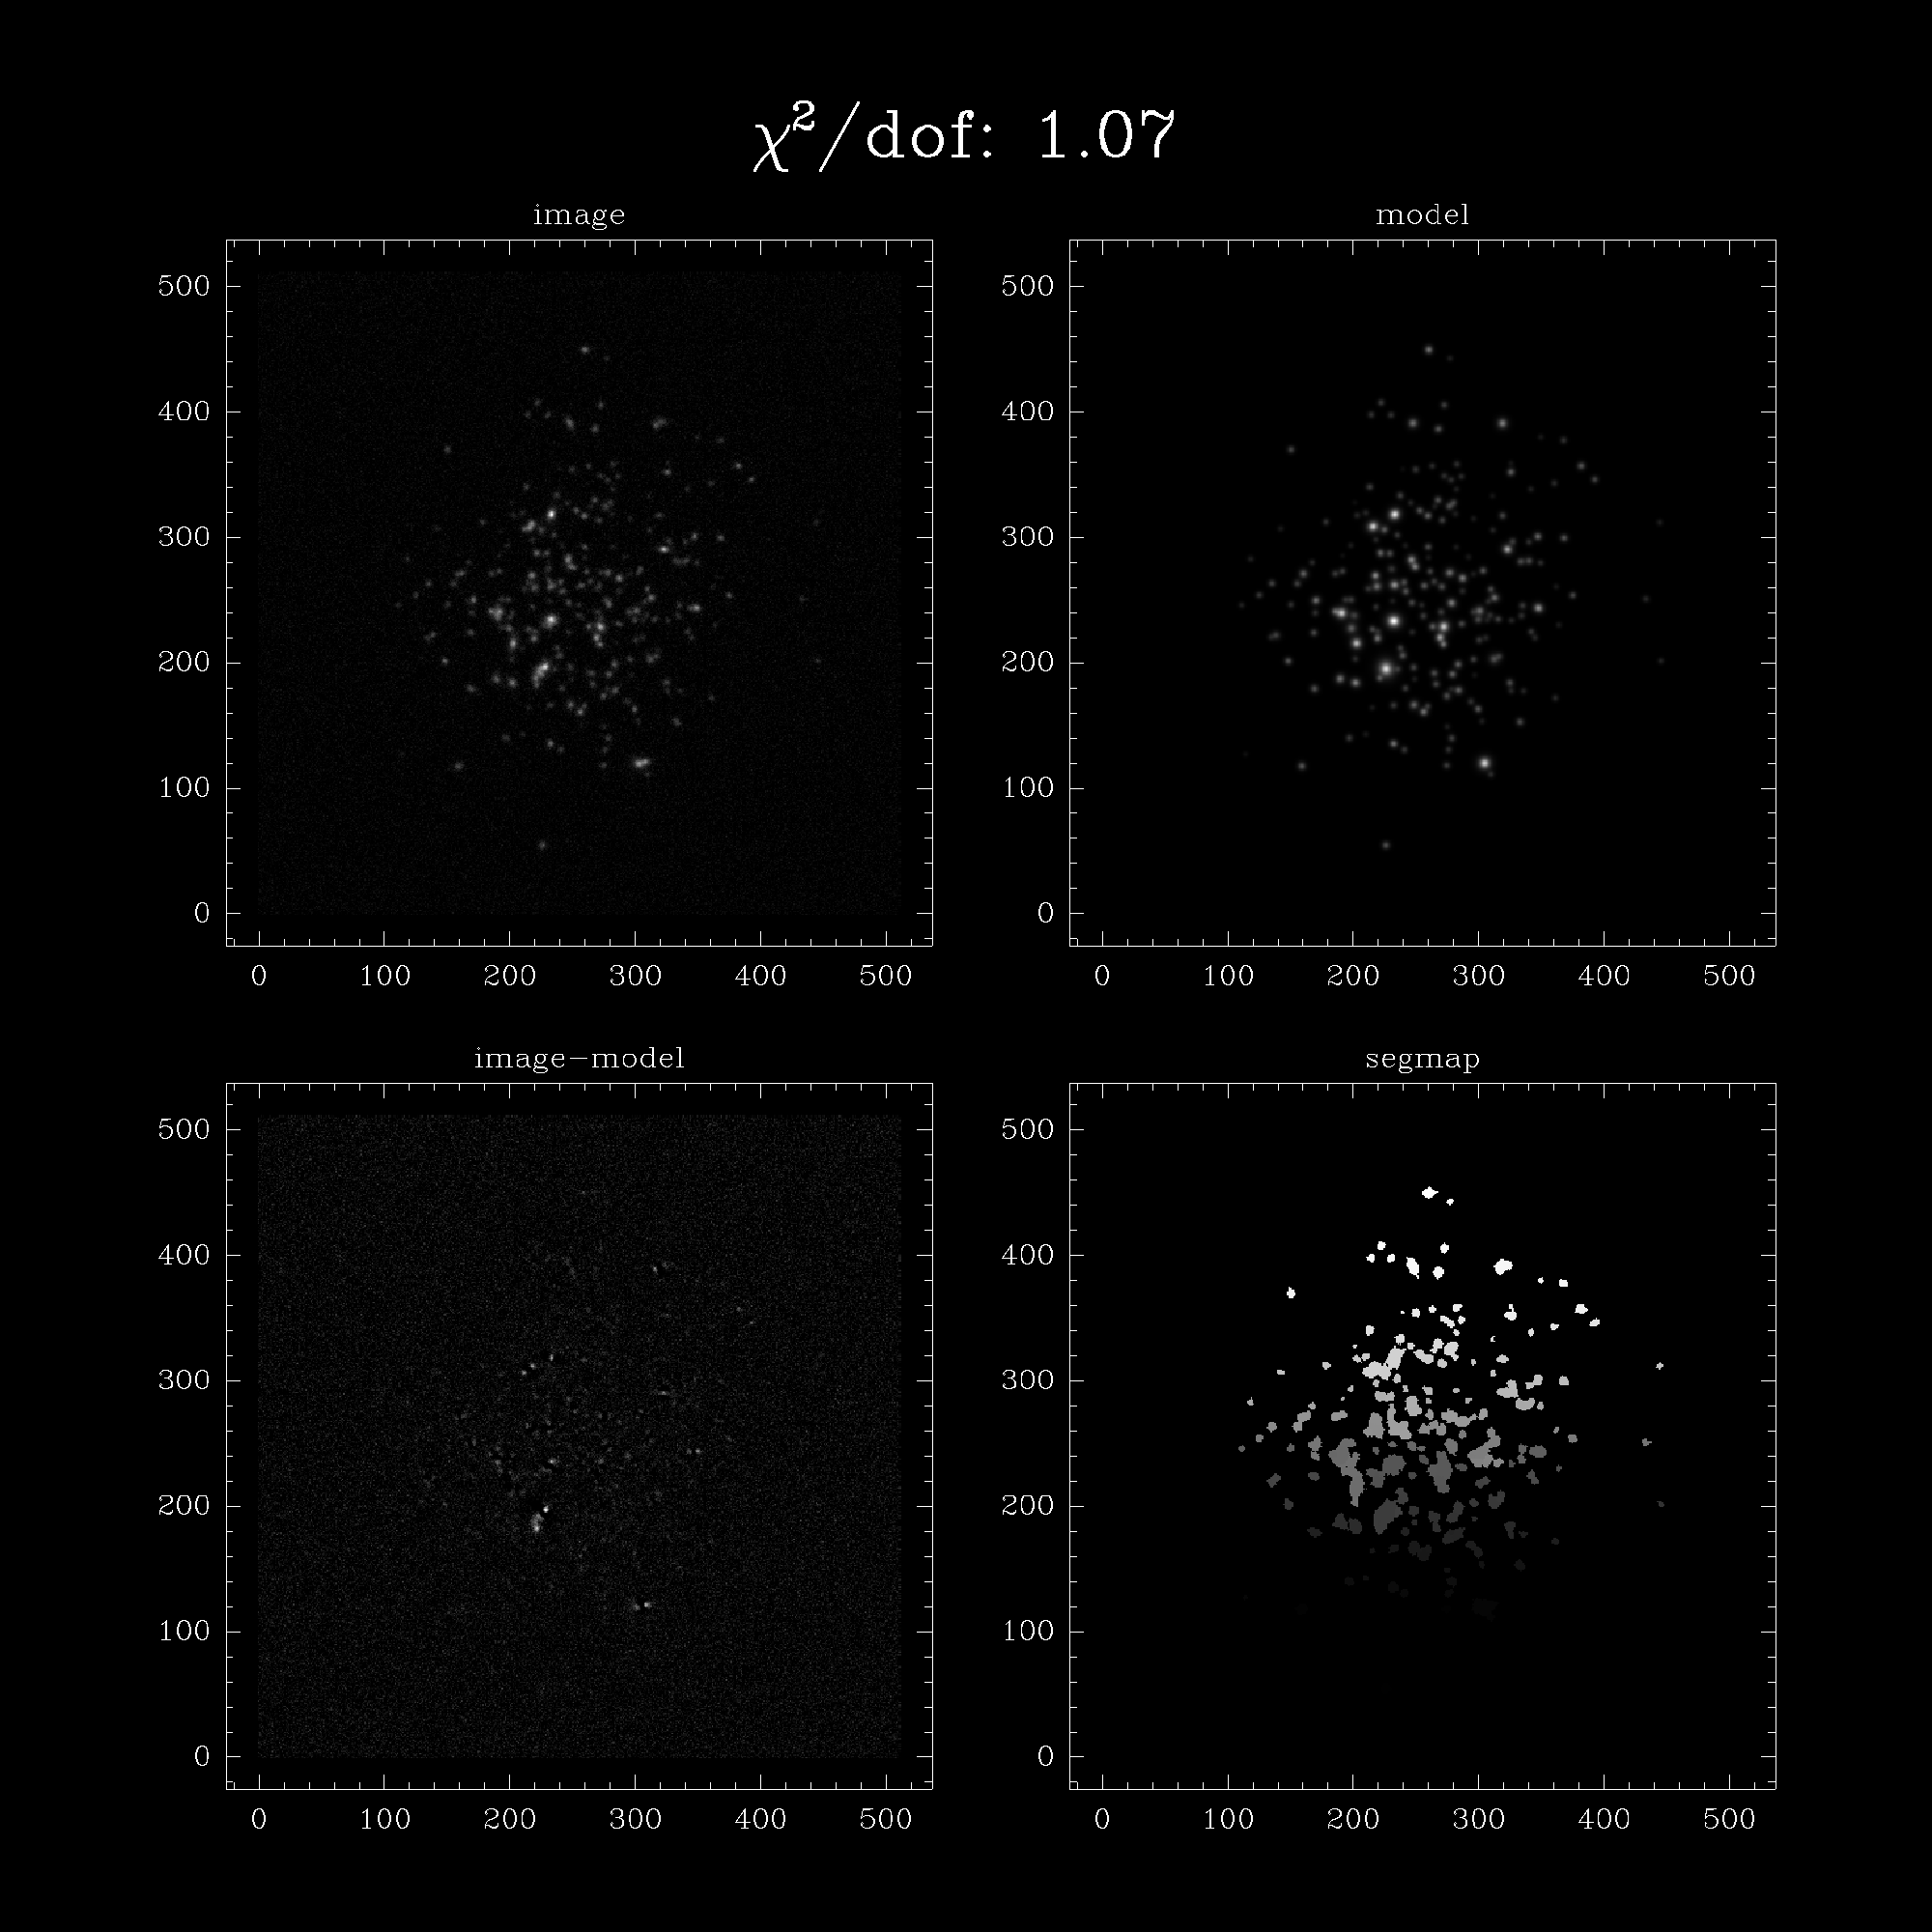
\includegraphics[trim={5cm 3cm 5cm 37cm},clip,width=\columnwidth]{diff-20855-000000.png}
    \end{center}
}


\end{document}
